\section{Interface Design}
\label{sec:sp-design}

\subsection{Approach}
The design process started with a close examination of the analysis steps we plan to support. For transcription, we ruled out the possibility of automatic video or audio transcribing because these are research challenges in their own right and require expertise different from visualization and visual analytics. During our meta observation data analysis, we noticed that a large portion of time spent on transcribing video recordings was to identify the sensemaking actions that the participants performed (such as searching) and contextual information associated with these actions (such as the search keyword and its timing). These pieces of information can potentially be captured within the browser, thus considerably reducing transcribing time.

From the aforementioned participatory design session, we found that an important part of the coding process is to understand the sensemaking activities from the video transcripts. For instance, when a participant spent several minutes on a page, he was likely reading through the information. When the participant switched between two pages back and forth, he might be comparing two smart watch models. Understanding the nature of such sensemaking activities; i.e., reading or comparison, is the prerequisite for identifying common themes and naming them. To a certain extent, this is equivalent to inferring ``sub-task'' from ``action'' in the Gotz and Zhou's model. However, this process is difficult to be completely automated~\cite{Dou2009}. After further discussion with the HCI researchers, we identified three important factors to this process that can be supported by visualization:
\begin{enumerate}
	\item \textbf{Seeing the actions before and after the current one}. This provides useful contextual information because an ``action'' is usually a part of a ``sub-task'', which consists of a number of actions. For example, when a participant went through the web page of a number of hotels in succession, they might be comparing these hotels, especially if all these pages are opened from the same hotel booking website. Showing a number of actions together would help a researcher to identify the connections between them and potentially find an interpretation for all the actions in the sequence as a whole.
	\item \textbf{Seeing what a participant was looking at}. It may appear obvious, but it can give a researcher the needed context to understand the sensemaking actions. For example, looking at Google Maps may indicate the participant was trying to locate a certain place. This can be particularly useful if the researcher is absent from the observation.
	\item \textbf{Understanding what a participant was thinking}. Even though this can be partly captured through think-aloud protocol or post hoc interview, another common technique is to enable participants to record their own thinking by providing note taking support.
\end{enumerate}

\subsection{Overview}
SensePath is designed as a Chrome extension consisting of two parts. The first one is a background process running in the participant's browser to automatically capture all the required analytic provenance during the observation stage of the qualitative study. It also offers additional features to add note and highlight text on a web page (Factor 3 -- understanding what a participant was thinking). Besides, participants will not notice any difference from their normal sensemaking session (Requirement 4 -- non-intrusiveness).

The second part is designed to facilitate transcription and coding (Requirement 1 and 2), including a set of four linked visualizations of the captured provenance data (\autoref{fig:sp-overview}) as follows.

\begin{itemize}
\item A \emph{timeline} view displaying participant's sensemaking actions in their temporal order (\autoref{fig:sp-overview}A). This enables researchers to see an action in the context of other actions (Factor 1 -- seeing the actions before and after the current one).
\item A \emph{browser} view showing the web page where the sensemaking action was performed (\autoref{fig:sp-overview}B). This provides the contextual information of sensemaking actions (Factor 2 -- seeing what a participant was looking at).
\item A \emph{replay} view showing screen capture video (\autoref{fig:sp-overview}C). This provides additional contextual information about browser interaction that is missing from the timeline such as scrolling and mouse movement (also Factor 2).
\item A \emph{transcription} view displaying details of selected sensemaking actions (\autoref{fig:sp-overview}D). The generated transcript can be exported and then used in popular qualitative data analysis software (Requirement 3 -- existing workflow integration).
\end{itemize}

\begin{figure}
 	\centering
 	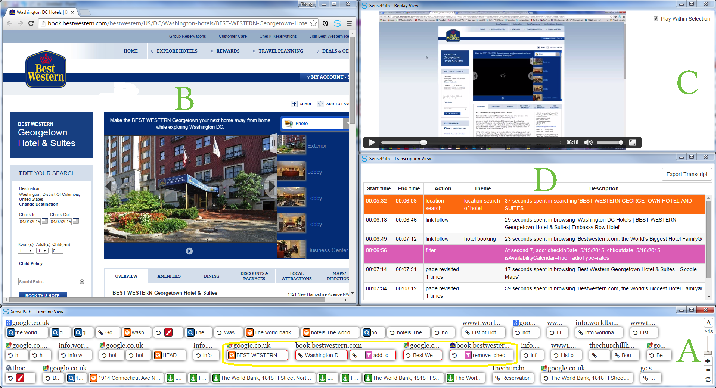
\includegraphics[width=\linewidth]{overview}
 	\caption[Four linked visualizations of SensePath]{Four linked visualizations of SensePath. \textbf{A:} The timeline view shows all captured sensemaking actions in temporal order. \textbf{B:} The browser view displays the web page where an action was performed. \textbf{C:} The replay view shows the screen capture video to provide additional context. \textbf{D:} The transcription view details selected actions (highlighted in the timeline) and generates their transcript.}
 	\label{fig:sp-overview}
\end{figure}

\subsection{Provenance Capture}
\label{sub:sp-provenance}
During the participatory design session, the HCI researchers suggested to capture rich semantic  information that is able to explain the rationale of actions the participant performed. However, this is not always technically feasible. For example, it is possible to detect that a web page has been opened for a long time, but it may be impossible to know whether the participant was reading, thinking, or simply away from the computer screen just by using the information available from the browser alone. Therefore, we agreed to capture the analytic provenance corresponding to the ``action'' level in the Gotz and Zhou's model. This capture can be done automatically yet still provides reasonable amount of semantics to the researchers. We decided to record the following aspects of actions that were regarded useful for qualitative analysis of sensemaking by the HCI researchers, as summarized in \autoref{fig:icon-list}.

\begin{itemize}
	\item \textbf{Type}: When a participant opens a web page, the default type for that action is \emph{browsing}, which lasts until the page becomes inactive. During that period, two common action types are focused: \emph{search \& filter} and \emph{reading}. The former type includes \emph{keyword search}, \emph{location search}, \emph{route search} and \emph{filter}. The latter type includes \emph{highlight} and \emph{annotation}, provided for taking notes and capturing part of the participant's thinking.

	\item \textbf{Timing}: This includes the start and end time of an action.

	\item \textbf{Context}: This contextual information provides additional clues for researchers when looking at individual actions. It varies according to its action type such as the ``keyword'' for search and the ``selected text'' for highlight. Also, the information common for all action types including title, URL, and a screenshot of the rendered web page are always recorded.

	\item \textbf{Relationship}: This provides how a web page was activated with four cases: \emph{revisit} an already opened page, directly \textit{link} from an existing page, manually \textit{type} a new address, and open from a \emph{bookmark}.
\end{itemize}

\begin{figure}
	\centering
	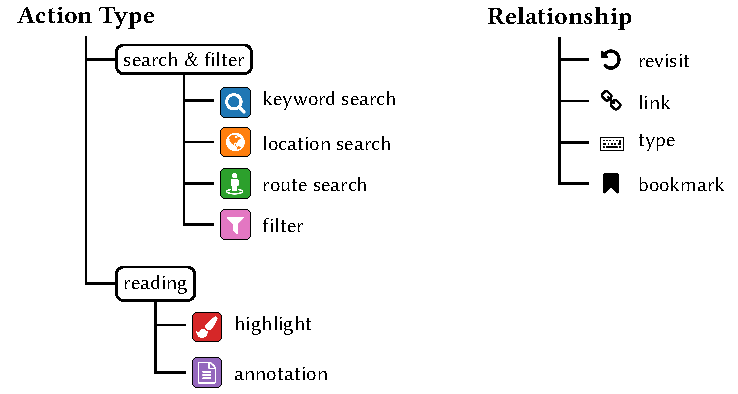
\includegraphics[width=\linewidth]{action-type}
	\caption[Action types and relationships]{All the action types and relationships that SensePath captures, next to the icons representing them.}
	\label{fig:icon-list}
\end{figure}

\subsection{Timeline View}
This view provides an overview of the entire sensemaking process, showing all the captured actions in their temporal order (\autoref{fig:sp-overview}A).

\subsubsection{Visual Representation}
An action is represented as either a bar or a tile, presenting all four aspects of provenance information discussed earlier.

\paragraph{Action Bar}
\autoref{fig:sp-action-bar} shows an example of an \textit{action bar}. The page URL (context) is displayed atop the bar. In the bar, the first icon shows that this action revisited a previously opened page (relationship). Next is the page title (context); only part of which is shown because of the limited space. This is followed by an icon indicating the type of that action such as a ``filter''. \autoref{fig:icon-list} shows all icons representing action types and relationships in SensePath. Note that action type icons have colored background and a black border to distinguish from relationship icons. The last part is the specialized context for each action type, which is filtering parameters in this figure. The width of the action bar corresponds to the length of time spent in browsing the web page, and the relative position of the action type icon marks when the action happened.

\begin{figure}
\centering
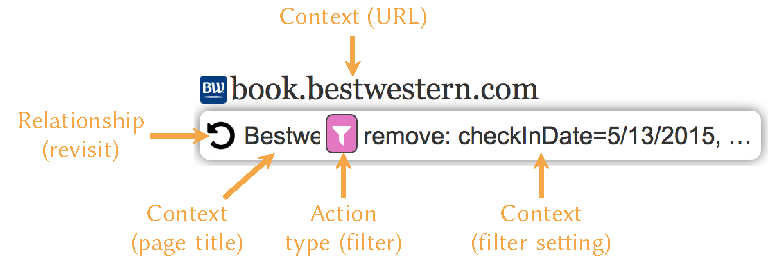
\includegraphics[width=\linewidth]{action-bar}
\caption[An action bar]{An action bar showing all four aspects of provenance information.}
\label{fig:sp-action-bar}
\end{figure}

\paragraph{Action Title}
An \emph{action tile} contains similar analytic provenance information but with more details. \autoref{fig:sp-action-tile} shows the same action as in \autoref{fig:sp-action-bar} but as a tile. Because more height is given, a tile includes a screenshot, which can help the researcher to recognize the web page more effectively. This can also be useful when the researcher was absent from the observation session because she may get a rough context of what the page was about by looking at the its thumbnail. The rest of the provenance information is the same as that in an action bar with more details (e.g., the page title) displayed because of the extra space.

\begin{figure}
\centering
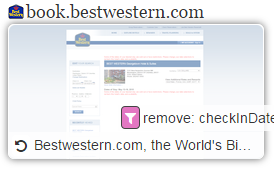
\includegraphics[width=.5\linewidth]{action-tile}
\caption[An action tile]{An action tile complementing the action bar with a page screenshot.}
\label{fig:sp-action-tile}
\end{figure}

The timeline can be shown with either action bars or tiles, interactively controlled by the user. The former is more compact and scalable, whereas the latter shows more details and is suitable for a close inspection. \autoref{fig:sp-timeline-tile} shows an example of timeline with action tiles.

\begin{figure}
\centering
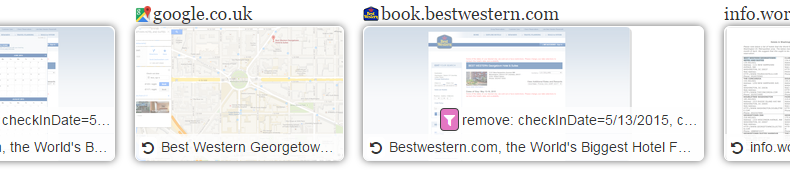
\includegraphics[width=\linewidth]{timeline-tile}
\caption{A part of the timeline with action tiles.}
\label{fig:sp-timeline-tile}
\end{figure}

\subsubsection{Scalability}
\paragraph{Zooming}
Both action bar and tile can reduce their widths through zooming to accommodate more actions. At the smallest level, only the action type is visible, and more details will become available when zooming in. \autoref{fig:sp-timeline-zoom} shows three zoom levels of action bars with the details increasing from top to bottom. The top row shows actions with only icons and a few letters. The middle row reveals the last location search is about ``Best Western'' hotel. The bottom row shows that the first location search is about some ``headquarters'', and the second action is revisiting the ``World bank'' web page. At a low level of detail, only a few letters are shown for each action bar, thus is uninformative. In this case, information richness is sacrificed for scalability. To mitigate this issue, we introduce interactive features such as \emph{selective zooming}, which will be discussed later.

\begin{figure}
\centering
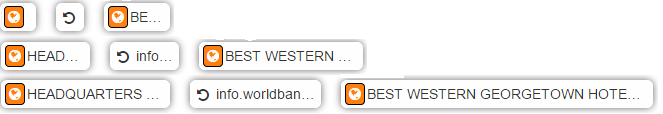
\includegraphics[width=\linewidth]{zoom-3levels}
\caption[Three zoom levels of action bars]{Three zoom levels of action bars with the details increasing from top to bottom.}
\label{fig:sp-timeline-zoom}
\end{figure}

\paragraph{Aggregate Actions}
Instead of showing individual actions, adjacent ones happened on the same web page are merged to save space. It may also help the researcher to quickly understand the participant's process. \autoref{fig:sp-action-bar-merge} shows an aggregated action with eight highlights, which were made on the same Google Plus page.

\begin{figure}
\centering
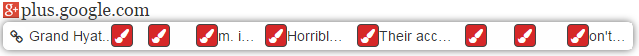
\includegraphics[width=\linewidth]{action-bar-merge-new}
\caption[An aggregate action bar]{An aggregate action bar. It combines eight adjacent highlights made on the same Google Plus page.}
\label{fig:sp-action-bar-merge}
\end{figure}

Because the action bar is short, a timeline can show multiple rows. This, in combination with aggregation and interaction (described next), enables SensePath to display a reasonably large sensemaking session within a limited space. \autoref{fig:sp-overview}A shows about 50 actions out of a total of 70 actions from a 30-minute long session. This addresses Requirement 5 on scalability.

\subsubsection{Interaction}
\paragraph{Mouse Click and Hover}
SensePath includes a number of interactive features to support the analysis of the sensemaking process. Clicking on an action opens the associated web page in the browser view (\autoref{fig:sp-overview}B). This enables researchers to see what the participant was looking at, which is a prerequisite for understanding their thinking. Hovering an action bar highlights other actions happened in the same page with a red border, and brings up a tooltip with additional details such as timing. The example in \autoref{fig:sp-hovering} shows that a page was revisited a number of times during a short sensemaking session.

\begin{figure}
\centering
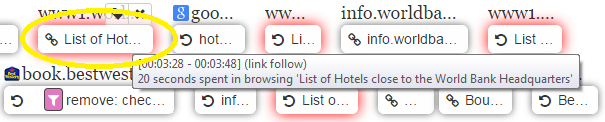
\includegraphics[width=\linewidth]{hovering}
\caption[Mouse hovering effect]{Mouse hovering effect. When an action bar is hovered (highlighted with a yellow eclipse), all other actions with the same URL (red borders) are also highlighted, and a tooltip is showing additional information.}
\label{fig:sp-hovering}
\end{figure}

\paragraph{Selective Zooming}
SensePath implements a focus+context technique~\cite{Cockburn2008} through \emph{selective zooming}: when a zoom is executed, only a selected set of actions affects. This enables researchers to concentrate on certain actions without losing their context. However, they may forget the difference in zoom levels of actions, thus misunderstand the action lengths indicated by the bar widths. SensePath provides a reset button to change the zoom levels of all actions to the default value. \autoref{fig:sp-selective-zooming} illustrates this technique.

\begin{figure}
\centering
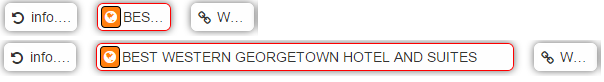
\includegraphics[width=\linewidth]{selective-zooming}
\caption[Selective zooming]{Selective zooming. Selected action bars are with red borders. Top row: before zooming. Bottom row: after zooming -- only the selected action has its zoom level changed.}
\label{fig:sp-selective-zooming}
\end{figure}

\paragraph{Filtering}
Researchers can filter actions based on duration, enabling them to focus on the range of actions they want. For example, if researchers think actions that last only a few seconds are trivial, they can be filtered out using a slider (\autoref{fig:sp-filter}), which sets a minimal length for visible actions. When the slider moves, actions that will be removed fade out, before disappearing when the slider stops. This enables researchers to preview the effect of filtering.

\begin{figure}
\centering
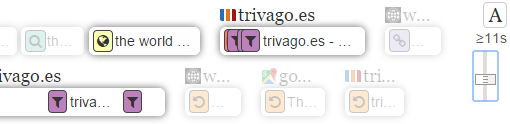
\includegraphics[width=\linewidth]{filter}
\caption[Actions filtering]{Actions filtering. The slider (on the right side) controls the minimal length visible actions. Actions fall below the threshold fade out first before completely disappearing.}
\label{fig:sp-filter}
\end{figure}

\paragraph{Coding}
In traditional qualitative analysis, researchers analyze transcripts to identify common themes and assign suitable names or codes to them. In SensePath, the timeline view provides a succinct summary of the sensemaking process and allows researchers to drill down to explore more specific actions. Representing action types with icons and visualizing a sequence of actions next together may also help researchers to quickly identify patterns of the data, compared to watching videos or reading transcripts. The coding feature is available through a menu button when hovering an action bar. Researchers can assign a code by simply typing it or selecting from a list of previously entered ones.

\subsection{Browser View}
\label{sub:webpage}
When an action is selected in the timeline, its associated web page is shown in the browser view (\autoref{fig:sp-overview}B). This enables researchers to examine the web page that the participant was looking at when performing a sensemaking action. If the action is an annotation or highlight, the browser view will automatically navigate to the location of the web page where the annotation or highlight was made, informing researchers which part of the page the participant was interested in.

\subsection{Replay View}
\label{sub:playback}
SensePath links the timeline to an externally captured screen video to provide additional information about the participant's behavior during the sensemaking session. When a researcher selects an action in the timeline, the replay view automatically jumps to the corresponding part of the screen video when the action is about to start. This avoids manual search within the video, which can be time consuming. After selecting an action in the timeline, a researcher can first check the web page in the browser view and then start the video playback in the replay view if she wants to find out more. The playback automatically stops when it reaches the end of an action, avoiding watching other irrelevant part. Alternatively, the researcher can choose to allow the video to continue; if so, the corresponding action in the timeline will be highlighted as the video progresses.

\subsection{Transcription View}
Detailed information of an action can be revealed by mouse over; however, it is inconvenient to do so for a set of actions. The transcription view addresses this issue by simultaneously presenting the details for all selected actions, in a tabular format (\autoref{fig:sp-overview}D). For each action, this view shows its starting and ending time, action type, assigned themes, and an automatically generated description such as ``37 seconds spent in searching Best Western George Town Hotel and Suites''. This description is based on a predefined template for each different action type with advise from the aforementioned participatory design session. The researchers are allowed to edit the description to better reflect what they think. Row backgrounds match the color of action type icons in the timeline view. The design of this view resembles the transcript interface of popular video transcription software packages to reduce the learning efforts required.

All the information displayed in the transcription view can be exported as a timeline in the SMPTE format~\footnote{ \url{http://en.wikipedia.org/wiki/SMPTE_timecode}}, which can be imported by many popular qualitative data analysis software packages such as InqScribe~\footnote{\url{http://www.inqscribe.com/}} as a transcript. This enables researchers to continue their existing workflows with such software (Requirement 3). Moreover, an SMPTE transcript can be used as a subtitle file in popular video players such as VLC~\footnote{\url{http://www.videolan.org/vlc/index.en_GB.html}}.

\subsection{Implementation}
\label{sub:sp-impl}
This section discuss the architectural design of SensePath and techniques in capturing and detecting provenance.

\subsubsection{Architecture}
SensePath is implemented as a Chrome extension using modern web technologies including HTML5, CSS3, JavaScript and D3.js~\cite{Bostock2011} for visualization. Therefore, it satisfies Requirement 6 about lightweight and support multiple operating systems. Highlight and annotation features require the modification of web page structure, thus they must be implemented as a browser plug-in. We decided to target the Chrome browser first due to its popularity.

SensePath consists of two components: provenance capture and provenance visualization. The capture component relies on content script injected into a loaded web page (to allow highlight and annotation) and the Chrome extension API (to allow automatic action extraction). Therefore, it always works as long as the Chrome extension is enabled. The captured data is exported as a JSON file, which can then be loaded into the visualization component.

The four linked visualizations communicate to each other using the \textit{messaging passing} mechanism provided by the Chrome extension API. When an interaction occurs in one view, it sends a message to notify all other views. Each view constantly listens and responds to such messages. For instance, when an action is selected in the timeline view, it broadcasts that selection. The replay view listens and changes the current time frame of the video to when that action was performed. The replay view uses HTML5 video tag~\footnote{\url{https://developer.mozilla.org/en-US/docs/Web/Guide/HTML/Using_HTML5_audio_and_video}} to display the video capture, thus possible to programmatically set the current playback position to a specific point and to start/pause the playback. The replay view also maintains a list of start/end time of all actions, thus when a video is playing, it finds the action that contains the current time frame and sends a message to the timeline view to highlight it.

\subsubsection{Provenance Capture Techniques}

\paragraph{Search}
Detecting all \emph{search} actions applies URL parsing. When a web page is loaded, its URL is parsed and compared against a set of query templates to check whether a search was performed and to identify its type and parameters. In this prototype, we support automatic detection from many popular web services: keyword search engines (Google, Yahoo, Bing, Ask.com and DuckDuckGo), map search engines (Google Maps, OpenStreetMap and Yahoo Maps), social networking websites (Facebook and Twitter), e-commerce websites (Amazon and ebay) and hotel booking websites (Booking.com and Expedia). All these web services follow their own query templates and expose all necessary parameters in the URLs, allowing extracting the required information from them. The following examples show the query templates and parameters:

\begin{itemize}
	\item Google keyword search: \texttt{https://www.google.com/search?\\\textbf{q=\{keyword\}}}
	\item Yahoo Maps route search: \texttt{https://maps.yahoo.com/directions?\\\textbf{o=\{source\}\&d=\{destination\}}}
\end{itemize}

SensePath uses a structure with three parameters to represent these templates, including a host name (\texttt{www.google.}), a path name (\texttt{/search}) and a regular expression (\verb|/\Wq=([\w%+]*)/i|) for keyword extraction. Adding detection support to other services only requires the knowledge of these three parameters.

\paragraph{Filter}
Detecting \emph{filter} actions also uses URL parsing as in detecting \emph{search} actions but does not require prior knowledge about query templates. We apply a heuristic that if two consecutive URL requests share the same host name and path name but different parameters, the second page is the result of a filtering action on the first one. More specifically, a URL is compared against its previous URL within the same tab; if they have the same host name and path name, their query strings are parsed to a collection of key/value pairs. For each key, three cases can happen when comparing its value between the previous and the current URL:

\begin{itemize}
	\item \textbf{add}: The key was absent from the previous URL but is added to the current one.
	\item \textbf{remove}: The key was present in the previous URL but is removed from the current one.
	\item \textbf{update}: The key is present in both URLs but their values are different. Note that if their values remain unchanged, it is unnecessary to report.
\end{itemize}

For example, considering these two consecutive URLs:
\begin{enumerate}
	\item \url{hotel.com/search?loc=london&guests=1}
	\item \url{hotel.com/search?loc=london&guests=2&in=2015%2F10%2F24}
\end{enumerate}

Following our heuristic of comparing URLs, this filter action can be captured as ``\texttt{add:} \texttt{\{in=2015/10/24\}, update:} \texttt{\{guests=1$\rightarrow$2\}}'', and may be interpreted as ``the participant set a new check-in date and changed the number of guests from 1 to 2''.

\paragraph{Limitations} Both \emph{highlight} and \emph{annotation} actions are implemented using the content script~\footnote{\url{https://developer.chrome.com/extensions/content_scripts}} in the Chrome extension API, thus all information needed can be saved. To allow revisiting to the exact location where a passage of text is highlighted, the relative location of its DOM element to the root element of the web page is captured. However, when the web page structure is changed, the recorded position might become invalid, leading to inaccurate recovery.

All the heuristics applied for search and filter actions only work if web services expose their parameters in the URL. In other words, our method fails to work if POST or AJAX requests are used. So far, for all services we planned to support, we have never encountered such a case. For example, Google Maps uses AJAX calls to load map tiles, but all the information we want to extract is available in the URL. Also, most popular online services use GET instead of POST requests. It is actually possible to support web services that encode the required information in POST or AJAX requests by monitoring all the communication between the browser and the server, not just the changes in URL. However, this requires considerably more implementation effort and is only possible with open source browsers such as Firefox and Chrome that provide access to all client-server communication.

For GET requests, it is also infeasible to extract the meaning of URL parameters if they are encoded. We encountered one such case, Bing Maps, which encodes query parameters as HEX strings. For example, this lengthy URL, \url{https://www.bing.com/maps/#Y3A9NTEuNTkwMTk5fi0wLjIyNTAw...}, \\is the URL produced by searching for ``london''.

To guarantee an exact restoration of a visited web page, it is necessary to save a static copy of the web page when an action happened. This is similar to the \emph{P-Set model}~\cite{Jankun-Kelly2007} for visualization exploration where the visual transforms, parameters, and results are stored for fully describing and reproducing the performed process. However, for simplicity, we only capture the action type (i.e., visual transforms) and context (i.e., parameters), but not the resulting web page (i.e., results). The browser snapshot and computer screen video are captured to compensate for this limitation to a certain extent.

\subsubsection{Trade-off in Provenance Capture}
The SensePath extension only captures user actions performed on the web browser, excluding all other types of provenance data to satisfy Requirement 6 -- lightweight. Screen capture can be done separately using another software such as QuickTime~\footnote{\url{https://support.apple.com/quicktime}}. Similarly, if the researchers have an interest in understanding which part of the screen a participant was looking at, eye tracking can be performed with an additional software. There might be no limit in capturing provenance information (such as face/gesture/brain tracking) for a comprehensive study of the sensemaking process performed by a participant. However, adding too many extra devices to capture provenance might affect the way participants perform their tasks. Therefore, we decided to take a lightweight approach to increase the application of SensePath.